\section{Zielsetzung}
    \noindent In diesem Versuch sollen verschieden Eigenschaften eines LRC-Kreises untersucht werden. Diese sind der Dämpfungswiderstand, der aus der 
    zeitabhängigen Amplitude bestimmt wird, und der Widerstand bei dem der aperiodische Grenzfall eintritt. \\
    Zusätzlich wird an einem
    Serienresonanzkreis noch die Frequenzabhängigkeit der Kondensatorspannung und die Frequenzabhängigkeit der Phase zwischen Erreger- und 
    Kondensatorspannung untersucht.
   

\section{Theoretische Grundlagen}


    \subsection{RLC-Kreis}


    \begin{figure}[H]
        \centering
        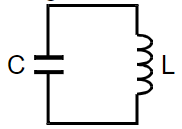
\includegraphics[width=0.2\textwidth]{images/unged.PNG}
        \caption{Ein ungedämpfter Schwingkreis\protect \cite{V354}.}
        \label{img:unged}
    \end{figure}

    \noindent In Abbildung \ref{img:unged} ist ein Schaltkreis aus einer Spule und einem Kondensator aufgezeichnet. Dies ist ein Schwingkreis 
    in dem der Strom ungedämpft zwischen den beiden Schaltelementen hin und her fließt.\\
    Wird in diesen Schwingreis noch ein Widerstand eingebaut, 
    entsteht ein gedämpfter Schwingkreis, wie in Abbildung \ref{img:gedKr} zu sehen. 
    In diesem Schwingkreis fällt die Amplitude konstant monoton.
    
    \begin{figure}[H]
        \centering
        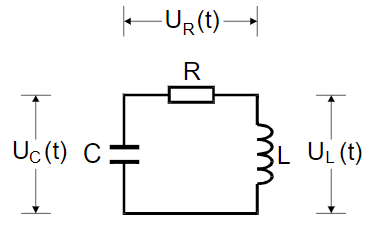
\includegraphics[width=0.3\textwidth]{images/gedKr.PNG}
        \caption{Ein gedämpfter Schwingkreis\protect \cite{V354}.}
        \label{img:gedKr}
    \end{figure}
    
    
    \subsection{Herleitung gedämpfter Schwingkreis}

    
    \noindent Zunächst wird nun eine Formel hergeleitet die gedämpfte Schwingkreise unterschiedlicher Formen beschreiben kann.
    Das 2. Kirchhoffsche Gesetz führt direkt zu einer Beziehung der abfallenden Spannungen:

    \begin{equation}
    U_{\symup{R}} + U_{\symup{C}} + U_{\symup{L}} +  = 0     
    \label{eq:Uabfall}
    \end{equation}

    \noindent In die Formel \ref{eq:Uabfall} lassen sich nun die für die Schaltelemente spezifischen Formeln einsetzten.
    \begin{align}
        U_{\symup{R}} & = RI \nonumber\\
        U_{\symup{C}} & = \frac{Q}{C}\nonumber\\
        U_{\symup{L}} & = L \cdot \symup{\frac{d}{dt}}I \nonumber
    \end{align}

    \noindent Dies führt zu einer Differentialgleichung der Form:
    \begin{align}
        L  \symup{\frac{d}{dt}}I + RI + \frac{Q}{C} & = 0 \nonumber\\
        \symup{\frac{d^2}{dt^2}}I + \frac{R}{L} \symup{\frac{d}{dt}}I + \frac{1}{LC}I & = 0 
        \label{eq:DGL1}
    \end{align}
    
    \noindent Diese Differentialgleichung wird über den Ansatz einer komplexen $\symup{e}$-Funktion gelöst.
    \begin{equation}
        I(t) = Z \cdot \symup{e}^{j \tilde{w} t}
        \label{eq:eAn}
    \end{equation}

    \noindent Einsetzen von \ref{eq:eAn} in die DGL \ref{eq:DGL1} ergibt:
    \begin{equation}
        \tilde{\omega}^2 - j \frac{R}{L}\tilde{\omega} - \frac{1}{LC} = 0 \nonumber
    \end{equation}

    \noindent Umstellen nach $\tilde{\omega}$ führt zu:
    \begin{equation}
        \tilde{\omega}_{1,2} = j \frac{R}{2L} \pm \sqrt{\frac{1}{LC}-\frac{R^2}{4L}} \nonumber
    \end{equation}
    
    \noindent $I(t)$ lässt sich nun also durch folgende Gleichung ausdrücken:
    \begin{equation}
        I(t) = Z_1 \cdot \symup{e}^{j \tilde{w}_1t} + Z_2 \cdot \symup{e}^{j\tilde{w}_2 t} \nonumber
    \end{equation}
    
    \noindent Die Definitionen für $\mu$ und $\nu$ bieten sich an um die Formel übersichtlicher zu gestalten.
    \begin{align}
        2 \pi \mu & \coloneq \frac{R}{2L} \nonumber\\ 
        2 \pi \tilde{\nu} & \coloneq \sqrt{\frac{1}{LC} - \frac{R^2}{4L^2}} \nonumber
    \end{align}

    \noindent $I(t)$ lässt sich dann als
    \begin{equation}
        I(t) = \symup{e}^{- 2 \pi \mu t} \cdot  (Z_1 \symup{e}^{j 2\pi \tilde{v}t} + Z_2 \symup{e}^{-j 2\pi \tilde{v} t}) \nonumber
    \end{equation}
    \noindent schreiben.\\
    Um $I(t)$ weiter zu unterschen muss  nun im folgenden eine Fallunterscheidung gemacht werden.
    Denn je nach dem ob der Inhalt der Wurzel positiv oder negativ ist, ist die Wurzel entweder reel oder imaginär. 
    \subsection{Fallunterscheidung}

        \subsubsection{1.Fall}
        Zu erst wird der Fall
        \begin{equation}
            \frac{1}{LC} > \frac{R^2}{4L^2}  \nonumber
        \end{equation}
        \noindent untersucht. \\
        Hier ist $v \in \mathds{R}$. Damit die Lösungsfunktion $I(t) \in \mathds{R}$ ist, muss
        $Z_1 = \overline{Z_2}$ sein. Dies lässt sich durch den Ansatz
        \begin{align}
            Z_1 & = \frac{1}{2} A_0 \symup{e}^{j \eta } \nonumber\\
            Z_2 & = \frac{1}{2} A_0 \symup{e}^{-j \eta} \nonumber
        \end{align}
        \noindent erreichen.
        
        \noindent Die folgende Identität, die die komplexe $\symup{e}$-Funktion enthällt:
        \begin{equation}
            \frac{\symup{e}^{j \phi} + \symup{e}^{-j \phi}}{2} = cos(\phi) \nonumber
        \end{equation}
        \noindent wird nun auf das Problem angewandt.

        \noindent Es ergibt sich damit:
        \begin{equation}
            I(t) = A_0 \symup{e}^{- 2 \pi \mu t} \cdot cos(2\pi \nu t + \eta) \nonumber
        \end{equation}
        \\
        \noindent Aus diesem Term kann nun eine Beziehung für die Periodendauer bestimmt werden:
        \begin{equation}
            T = \frac{1}{\nu} = \frac{2 \pi}{\sqrt{\frac{1}{LC}-\frac{R^2}{4L^2}}} \nonumber
        \end{equation}

        \noindent Mit der Näherung
        \begin{equation}
            \frac{1}{LC} \gg \frac{R^2}{4L^2} \nonumber
        \end{equation}

        \noindent entsteht hier die Thomsonsche Schwingungsformel
        \begin{equation}
            T_0 = \frac{2\pi}{\omega_0} = 2\pi \sqrt{LC} \nonumber
        \end{equation}

        \noindent Die Zeit $T_{\text{exp}}$ beschreibt den Zeitraum in dem die Amplitude auf den $\symup{e}$-ten Teil abfällt.
        \begin{equation}
            T_{\text{exp}} = \frac{1}{2 \pi \mu } = \frac{2L}{R} \nonumber
        \end{equation}

        \begin{figure}[H]
            \centering
            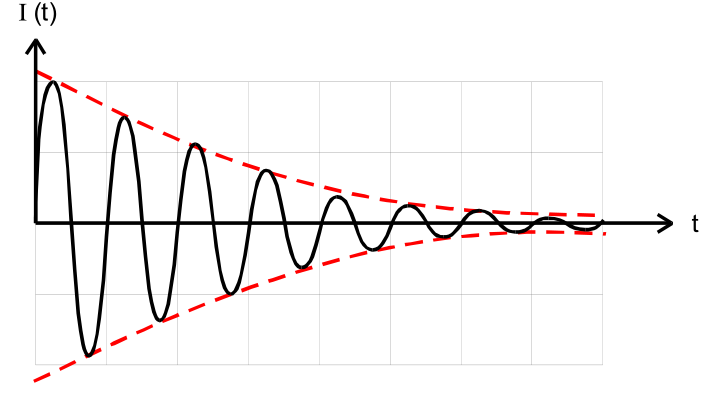
\includegraphics[width=0.7\textwidth]{images/ged.PNG}
            \caption{Ein Plot in dem eine gedämpfte Schwingung inklusive der einhüllenden Funktion skizziert ist\protect \cite{V354}.}
            \label{img:gedSch}
        \end{figure}

        \noindent In diesem exemplarischen Plot einer gedämpften Schwingung wird die rote Einhüllende durch den 
        exponential Term $A_0 \symup{e}^{- 2 \pi \mu t}$ und die Schwingung durch den cosinus Term $cos(2\pi \nu t + \eta)$ beschrieben.


        \subsubsection{2. Fall}


        \noindent Der zweite Fall beschreibt:
        \begin{equation}
            \frac{1}{LC} < \frac{R^2}{4L^2} \nonumber
        \end{equation}

        \noindent Hier ist dann $\tilde{v} \in \mathds{C}$.
        Für große Zeiten ergibt sich die Proportionalität:
        \begin{equation}   
            I \sim \symup{e}^{- \left( \frac{R}{2L} - \sqrt{\frac{R^2}{4L^2} - \frac{1}{LC}}\right) t} \nonumber
        \end{equation}

        \noindent Ein Spefzialfall für diesen Fall ist:
        \begin{equation}
            \frac{1}{LC} = \frac{R^2_{\text{ap}}}{4L^2} \nonumber
        \end{equation}
        
        \noindent Dadurch ist dann $\nu = 0$ und somit
        \begin{equation}
            I(t) = A \symup{e}^{-\frac{R}{2L}t} = A \symup{e}^{-\frac{t}{LC}} \nonumber
        \end{equation}

        \begin{figure}[H]
            \centering
            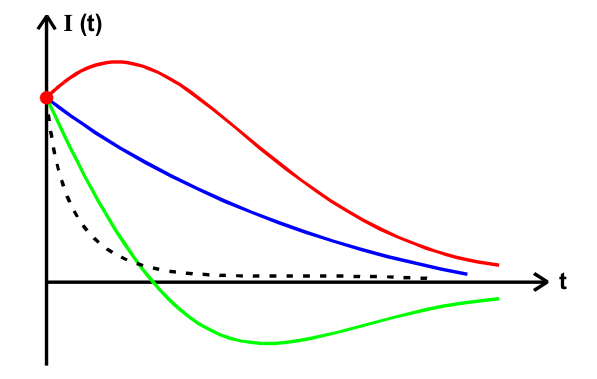
\includegraphics[width=0.7\textwidth]{images/AperiodischD.PNG}
            \caption{Ein Plot mit unterschiedlich abfallenden Funktionen \protect \cite{V354}.}
            \label{img:aperi}
        \end{figure}

        \noindent Den in Abbildung \ref{img:aperi} durch die gestrichelte Linie beschriebene Funktion, wird als Aperiodischer Grenzfall 
        bezeichnet. Dies ist der Fall in dem die Amplitude am schnellsten und ohne nachfolgende Schwingungen auf 0 absinkt.

        %\subsection{Vergleich Mechanik}


       % Hier bietet sich nun ein Vergleich mit einer rein mechanischen Schwingung an.
       % 
       % \begin{equation}
       %     m \ddot{x} + s \dot{x} + Dx = 0 \nonumber
       % \end{equation}
       %
       % \begin{align}
       %     m \Leftrightarrow L  \nonumber\\
       %     s \Leftrightarrow R  \nonumber\\
       %     D \Leftrightarrow \frac{1}{C} \nonumber
       % \end{align}

    \subsection{Erzwungene Schwingungen}
    

    \noindent In diesem Abschnitt werden LRC-Schwingkreise untersucht die von außen angeregt werden. 
    Dazu wird, wie in Abbildung \ref{img:erz} dargestellt,
    eine Spannungsquelle, die eine sinusförmige Spannung liefert, an einen Stromkreis angeschlossen.
    
    \begin{figure}[H]
        \centering
        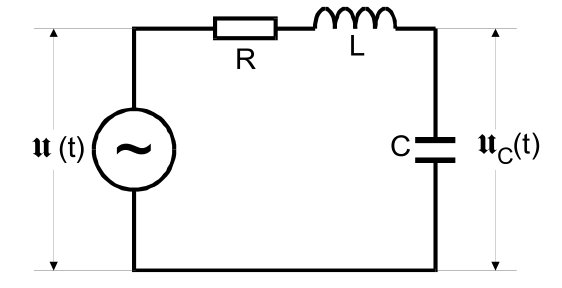
\includegraphics[width=0.7\textwidth]{images/Erzwungene.PNG}
        \caption{Schaltzeichnung einer erzwungenen Schwingung\protect \cite{V354}.}
        \label{img:erz}
    \end{figure}

    \begin{equation}
        u(t)= \symup{U_0} \symup{e}^{j \omega t} \nonumber
    \end{equation}
    $u(t)$ ist hierbei die anregende Spannung.

    \noindent Die Differentialgleichung hat nun also die Form:
    \begin{equation}
        L \dot{I} + R I + \frac{Q(t)}{C} = \symup{U_0} \symup{e}^{j \omega t} \nonumber
    \end{equation}

    \noindent Durch einsetzen des folgenden Terms 
    \begin{equation}
        V_{\symup{C}} (t) = \frac{Q(t)}{C} \nonumber
    \end{equation}

    \noindent ergibt sich dann:
    \begin{equation}
        LC \ddot{V}_{\symup{C}} + RC \dot{V}_{\symup{C}} + V_{\symup{C}} = \symup{U_0} \symup{e}^{j \omega t} 
        \label{eq:angDGL}
    \end{equation}

    \noindent mit $A \in  \mathds{C}$ als Amplitude der Kodensatorspannung.
    \begin{equation}
        u_{\symup{C}} (t) = A(\omega) \symup{e}^{j \omega t} 
        \label{eq:uteAn}
    \end{equation}

    \noindent Einsetzen von \ref{eq:uteAn} in \ref{eq:angDGL} liefert:
    \begin{equation}
        -LC \omega^2 A + j\omega RC A +A = \symup{U_0} \nonumber
    \end{equation}

    \noindent Die Formal nach $A$ umgestellt ergibt dann:
    \begin{equation}
        A= \frac{\symup{U_0}}{1 - LC \omega^2 + j \omega RC} = \frac{ \symup{U_0}(1 -LC \omega^2 - j\omega RC)}{\left( 1- LC \omega^2 \right)^2} \nonumber
    \end{equation}
    
    \noindent oder
    \begin{equation}
        |A|= \symup{U_0} \sqrt{\frac{\left(1-LC\omega^2\right)^2 + \omega^2 R^2C^2}{\left( \left(1 -LC \omega^2\right)^2 +w^2R^2C^2 \right)^2}}
        \label{eq:betA}
    \end{equation}

    \noindent Die Phase berechnet sich zu:
    \begin{equation}
        \text{tan}(\phi (\omega)) = \frac{\text{Im}(A)}{\text{Re}(A)} = \frac{\omega RC}{1 - LC\omega^2} \nonumber
    \end{equation}

    \noindent bzw.
    \begin{equation}
        \phi (\omega) = \text{arctan}\left(\frac{\omega RC}{1 - LC\omega^2} \right)
        \label{eq:phi}
    \end{equation}

    \noindent Da der Betrag der gesuchten Lösungsfunktion $u_{\symup{c}}(t)$ nach \ref{eq:uteAn} gleich dem Betrag von A ist, entsteht aus 
    \ref{eq:betA} das Ergebnis:
    \begin{equation}
        U_{\symup{C}}(\omega) = \frac{U_0}{\sqrt{\left(1-LC\omega^2)\right)^2 + \omega^2 R^2 C^2}} 
        \label{eq:Ucw}
    \end{equation}

    \noindent Somit ist die gesucht Funktion für $U_{\symup{C}}$ in Abhängigkeit von $\omega$, der Frequenz der Erregerspannung, gefunden.\\
    Durch weiteres Untersuchen von \ref{eq:Ucw} ergibt sich, dass $U_{\symup{C}}$ für $\omega \to \infty $ gegen 0 und für $\omega \to 0$ gegen 
    das $U_0$ der Erregerspanung geht.\\
    Jedoch gibt es auch ein $\omega$ bei dem das $U_{\symup{C}}$ ein Maximum erreicht, welches die 
    Erregerspannung übertrifft. Dieses Phänomen wird als Resonanz bezeichnet und tritt bei der Resonanzfrequenz $\omega_{\text{res}}$ ein. \\\\
    \noindent
    Berechnungen ergeben als Formel für $\omega_{\text{res}}$:
    \begin{equation}
        \omega_{\text{res}} = \sqrt{\frac{1}{LC}-\frac{R^2}{2L^2}} \nonumber
    \end{equation}
    \newline
    \noindent
    Für: 
    \begin{equation}
        \frac{R^2}{2L^2} \ll \frac{1}{LC} \nonumber
    \end{equation}

    \noindent ergibt sich ein Fall von besonderer Bedeutung. Für diesen Fall nähert sich $\omega_{\text{res}}$ nämlich an $\omega_0$, der Frequenz einer ungedämpften 
    Schwingung, an.\\
    In diesem Fall übertrifft $U_{\symup{C}}$ die Erregerspannung.
    \begin{equation}
        U_{\text{C,max}} = \frac{1}{\omega_0 RC} = \frac{1}{R} \sqrt{\frac{L}{C}} U_0 \nonumber
    \end{equation}

    \noindent Somit kann $U_{\symup{C},\text{max}} \to \infty$ für $R \to 0$ gehen. Dies wird als \enquote*{Resonanzkatastrophe} bezeichnet. Der Faktor
    $\frac{1}{\omega_0 RC}$ wird auch als als Resonanzüberhöhung oder Güte q des Schwingkreises bezeichnet. Die Schärfe der Resonanz 
    der Resonanzkurve wird durch die Schnittpunkte $\omega_{\pm}$, die jeweils den Ort an dem $U_{\symup{C}}$ auf einen Faktor $\frac{1}{\sqrt{2}}$ 
    absinkt, beschrieben.\\
    Somit werden $\omega_+$ und $\omega_-$ durch 
    \begin{equation}
        \frac{U_0}{\sqrt{2}} \frac{1}{\omega_0 RC} = \frac{U_0}{C \sqrt{\omega^2_{\pm} R^2 + \left( \omega^2_{\pm}L - \frac{1}{C} \right) }} \nonumber
    \end{equation}
    beschrieben.\\

    \noindent Für $\frac{R^2}{L^2} \ll {\omega}^2_0$ folgt für die Breite der Resonanzkurve:
    \begin{equation}
        \omega_+ - \omega_- \approx \frac{R}{L} 
        \label{eq:v1}
    \end{equation}

    \noindent Somit besteht auch folgende Beziehung zwischen der Güte und der Breite:
    \begin{equation}
        q = \frac{\omega_0}{\omega_+ - \omega_-} \nonumber
    \end{equation}

    \noindent Im Gegensatz dazu ist im Fall der starken Dämpfung:
    \begin{equation}
        \frac{R^2}{2L^2} \gg \frac{1}{LC} \nonumber
    \end{equation}

    \noindent Hier fällt jetzt die Spannung $U_{\symup{C}}$, ausgehend von $U_0$, mit steigender Frequez $\omega$ gegen 0. Bei hohen Frequenzen fällt
    die Spannung proportional zu $\frac{1}{\omega^2}$. Unter diesen Umständen kann der RLC-Kreis auch als Tiefpass benutzt werden.
    %\begin{equation}
    %    \omega^2_0 = \frac{1}{LC} \nonumber
    %\end{equation}
    \\\\
    \noindent Als nächstes wird die Frequenzabhängigkeit der Phase untersucht. Aus \ref{eq:phi} ist zu erkennen, dass für kleine $\omega$ die 
    Kondensatorspannung und die Erregerspannung fast in Phase sind, jedoch bei hohen Frequenzen $U_{\symup{C}}$ eine etwa um $\pi$ 
    kleinere Phase als $U$ hat.\\
    $\phi=\frac{-\pi}{2}$ gilt an der Stelle $\omega^2_0 = \frac{1}{LC}$.
    Aus \ref{eq:phi} folgt ebenfalls, dass $\omega_{1,2}$, bei denen $\phi= \frac{\pi}{4} \text{ oder } \frac{3\pi}{4}$ ist, folgende Beziehung erfüllen:
    \begin{equation}
        \omega_{1,2} = \pm  \frac{R}{2L} + \sqrt{\frac{R^2}{4L^2}+ \frac{1}{LC}} \nonumber
    \end{equation}

    \noindent Daraus folgt dann auch:
    \begin{equation}
        \omega_1 - \omega_2 = \frac{R}{L} 
        \label{eq:v2}
    \end{equation}

    \noindent Somit ist im Vergleich von \ref{eq:v1} und \ref{eq:v2} zu sehen, dass im Falle schwacher Dämpfung $\omega_1$ und $\omega_2$ 
    mit $\omega_+ - \omega_-$ zusammenfallen.


    \section{Impedanz des Schwingkreises}


        \subsection{Serienschwingkreis}

        
        \begin{figure}[H]
            \centering
            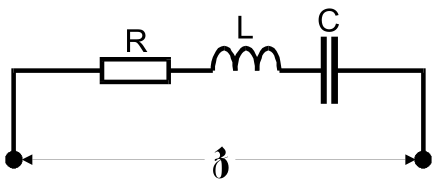
\includegraphics[width=0.7\textwidth]{images/Zweipol.PNG}
            \caption{Der Serienschwingkreis als Zweipol, hier wird die Impedanz als $r$ definiert\protect \cite{V354}.}
            \label{img:zweip}
        \end{figure}

    \noindent Ein Schwingkreis lässt sich auch, wie in Abbildung \ref{img:zweip} zu sehen, als Zweipol beschreiben.\\
    An seinen Enden kann nun ein frequenzabhängiger Widerstand $r$ gemessen werden Dieser wird als Impedanz bezeichnet.\\ 
    Aufgrund der Phasenverschiebung zwischen der Spannung 
    und dem Strom muss $r$ als komplexe Zahl definiert werden :
    \begin{equation}
        r = X + jY \nonumber
    \end{equation}

    \noindent Hier sind $X$ und $Y$ reele Widerstände, $X$ ist  der Wirkwiderstand und $Y$ ist der Blindwiderstand oder die Reaktanz. Der Betrag
    \begin{equation}
        |r| = \sqrt{X^2 + Y^2} \nonumber
    \end{equation}
    \noindent wird als Scheinwiderstand bezeichnet. In der komplexen Zahlenebene wird der Verlauf der Größe r($\omega$) als Ortskurve bezeichnet.\\
    $r$ ist dort nun ein Pfeil vom Ursprung dessen Länge der Scheinwiderstand und der Winkel zur reelen Achse die Phasenverschiebung 
    beschreibt.

    \begin{figure}[H]
        \centering
        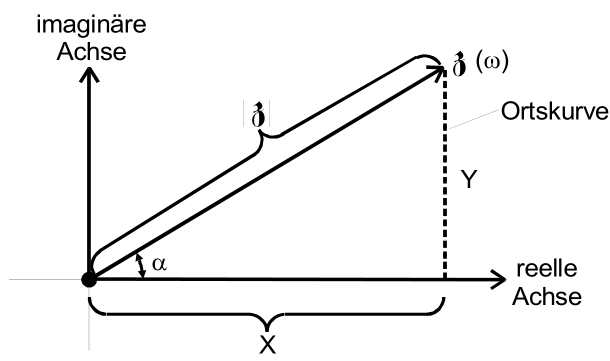
\includegraphics[width=0.4\textwidth]{images/Imaginaer.PNG}
        \caption{Eine Darstellung der Impedanz in der komplexen Zahlenebene\protect \cite{V354}.}
        \label{img:imag}
    \end{figure}

    \noindent Da die Elemente des Schwingkreises in Reihe geschalten sind wird dieser als Serienschwingkreis bezeichnet. Die gesamt Impedanz $r$ berechnet 
    sich durch die Impedanzen der einezlnen Bauteile:
    \begin{align}
        r_{\symup{C}} = -j\frac{1}{\omega C} \nonumber\\
        r_{\symup{L}} = j\omega L  \nonumber\\
        r_{\symup{R}} = R_{\symup{s}} \nonumber
    \end{align}

    \noindent Die gesamt Impedanz $r_{\symup{S}}$ berechnet sich also zu:
    \begin{equation}
        r_{\symup{S}} = R_{\symup{S}} + j \left(    \omega L - \frac{1}{\omega C} \right) \nonumber
    \end{equation}

    \noindent Aufteilung in real und imaginär Teil ergibt:
    \begin{align}
        X_{\symup{S}} = R_{\symup{S}}  \nonumber\\ 
        Y_{\symup{S}} = j \omega L - \frac{1}{\omega C} \nonumber
    \end{align}

    \noindent Damit ist
    \begin{equation}
        |r_{\symup{S}}| = \sqrt{R^2_{\symup{S}} + \left( \omega L - \frac{1}{\omega C} \right)^2} . \nonumber
    \end{equation}

    \noindent Da $X_{\symup{S}}$ nicht von $\omega$ abhängig ist schneidet die Ortskurve die x-Achse an der Stelle $R_{\symup{S}}$. Der Scheinwiderstand 
    selber ist bei $\omega = \omega_0 = \frac{1}{\sqrt{LC}}$ am geringsten, wächst jedoch bei $\omega \to 0$ und bei $\omega \to \infty$ 
    gegen $\infty$.


        \subsection{Parallelschwingkreis}
    
    
        \begin{figure}[H]
            \centering
            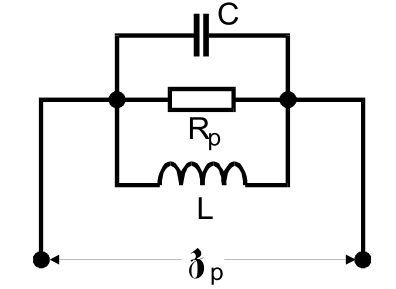
\includegraphics[width=0.3\textwidth]{images/Parallelschaltung.PNG}
            \caption{Schaltzeichnung eines Parallelschwingkreises, Impedanz wird hier als $r_{\symup{P}}$ bezeichnet.}
            \label{img:para}
        \end{figure}

        \noindent Die Impedanz $r_{\symup{p}}$ des Parallelschwingkreises wie in Abbildung \ref{img:para} berechnet sich zu:
        
    \begin{equation}
        r_{\symup{p}} = \frac{\frac{1}{R_{\symup{p}}}+j \left( \frac{1}{\omega L} - \omega C \right)}{\frac{1}{R^2_{\symup{p}}}+ \left( \frac{1}{\omega L} - \omega C \right)^2}
        \label{eq:Kreis}
    \end{equation}

    \noindent und somit der Scheinwiderstand zu:
    \begin{equation}
        |r_{\symup{p}}|=  \frac{1}{\sqrt{\frac{1}{R^2_{\symup{p}}} \left( \frac{1}{\omega L} - \omega C \right)^2}} \nonumber
    \end{equation}

    \begin{figure}[H]
        \centering
        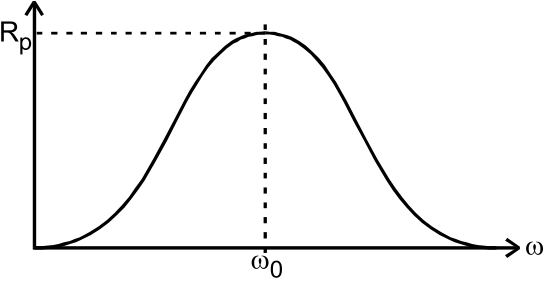
\includegraphics[width=0.7\textwidth]{images/Scheinwiderstand.PNG}
        \caption{Der Scheinwiderstandes in Abhängigkeit von der Frequenz in einem $R-\omega$ - Diagramm aufgezeichnet\protect \cite{V354}.}
        \label{img:scheinw}
    \end{figure}

    \noindent Hier ist zu sehen, dass bei der Resonanzfrequenz $\omega_0 = \frac{1}{\sqrt{LC}}$ der Scheinwiderstand im Gegensatz zum 
    Serienschwingkreis am größten wird, mit dem Widerstand $R_{\symup{P}}$ \ref{img:scheinw}.\\
    Er ist jedoch bei $\omega \to 0$ und bei $\omega \to \infty$ 
    vernachlässigbar. Gleichung \ref{eq:Kreis} ergibt ebenfalls, dass die Ortskurve des Parallelresonanzkreis die Form eines Kreises 
    mit dem Radius $\frac{R_{\symup{P}}}{2}$ und dem Mittelpunkt $\left( \text{0 , } \frac{R_{\symup{P}}}{2} \right)$ hat.\\
    Dies wird noch einmal im folgenden dargestellt.

    
    \begin{figure}[H]
        \centering
        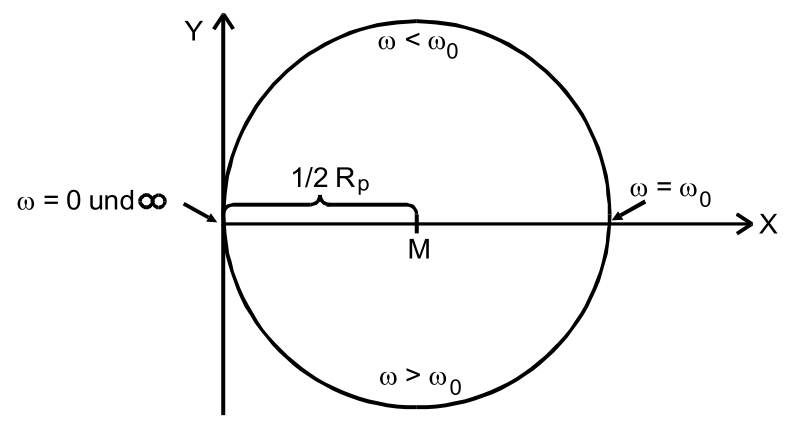
\includegraphics[width=0.7\textwidth]{images/Ortskurve.PNG}
        \caption{Ortskurve eines Parallelresonanzkreises.\protect \cite{V354}}
        \label{img:orts}
    \end{figure}
